
\section{Profilling Tool in PlanetLab}
\label{sec:planetlab}
In this section, the motivation for the use of \pl is explained together
with the design of the real system. Then, the platform and tools used are
described with their roles in the experiment. In addition, the network and
experiment design are broadly discussed. The execution of the experiment is also
presented. Finally, conclusions of this implementation are included.


\subsection{Definitions}
\begin{itemize}
\item\emph{Effective bandwidth (Mbps)} is the actual bandwidth at which the data
  can be transmitted on a link. The nominal bandwidth cannot be reached due to
  network congestion, the distance between nodes, delays, etc. Effective bandwidth is higher when nodes are closer, the congestion is scarce and the delays in the transmission are not long.
\item\emph{Bandwidth of the network(Mbps)}, which is the nominal ``width'' of the channel used, if the bandwidth increases, more data can simultaneously be sent, reducing the necessary time to transfer a packet of data. It is usually confused with the signal velocity, which affects the time the data takes to travel to the receiver (latency) but bandwidth cannot reduce this time.
\item\emph{Loss rate} is the fraction of data lost in the communication with respect
to all the data sent. It is a value between 0 and 1. It can also be provided in
percentage.

\item\emph{Latency (ms)} is the time it takes a signal to travel from its source, trough the communication channel, until it reaches the receiver. It is related with the distance between the nodes, the network congestion and the propagation velocity (a fraction of the light speed) among other parameters.
\end{itemize}

\subsection{Platform description}

The experiment presented was completely carried out in \pl, although the results obtained will be used to implement a realistic model of the networks in the communications between the simulators and the cloud system of the GEO-Cloud experiment implemented in \vw and \bonfire respectively.

\pl is a global research network that supports the development of new network
services~\cite{Europe2014}. This testbed currently consists of 1188 nodes at 582
sites, which allows researchers to develop new technologies for distributed
storage, network mapping, peer-to-peer systems, distributed hash tables and
query processing. Currently it is split into two platforms: \emph{PlanetLab
  Europe} that contains the European nodes and \emph{PlanetLab Central} which
contains the nodes located outside Europe.
For the experiment we use nodes from both of them.

\subsection{Tools description}

To implement and execute the experiment we use the following tools:
\begin{itemize}
\item \emph{NEPI}~\cite{INRIA2014}: it is a Python-based language library used to design and easily run network experiments on network evaluation platforms (e.g. \emph{PlanetLab}, \emph{OMF}, wireless testbeds and network simulators among others). It facilitates the definition of the experiment workflow, the automatic deployment of the experiment, resource control and result collection; and has the functionalities of automatic provisioning of resources and automatic deployment of the experiment. In the experiment \emph{NEPI} is used to provision the nodes and execute the whole experiment.
\item \emph{Iperf}~\cite{Iperf2014}: it is a tool used to measure the maximum
  \emph{TCP} bandwidth, allowing the tuning of various parameters and \emph{UDP}
  characteristics. \emph{Iperf} reports \emph{bandwidth},
  \emph{delay},\emph{jitter} and \emph{datagram loss}. This software allows any
  host to play the client and server roles. In the experiment, it was used to obtain the bandwidth with a step of one second when executed in \emph{TCP} mode and the loss rate when executed in \emph{UDP} mode. The nodes in Layer 1 and 2 were configured as clients and the cloud node as server.
\item \emph{Ping}~\cite{Pelsser2013}: It is
  software used to test if a host on an Internet Protocol is reachable. It
  measures the \ac{RTT} for messages sent from the originating host to a
  destination host. In the experiment, it was used to measure the latency
  delivery  of a package over the Internet between the nodes in Layer 1 and 2 and the central node.
\end{itemize}

\subsection{PlanetLab Experiment}

The objective of the \emph{GEO-Cloud} experiment is to simulate as realistically as possible the behaviour of a complete Earth Observation system~\cite{Gonzalez2014}. With this aim, the communication links in the real system have to be modelled to connect the simulators implemented in \vw and \bonfire with the values obtained from the experiment in \emph{PlanetLab}. The experiment then consists of communicating 12 real nodes representing the ground stations (the nearest \pl node to the real ground station was selected) and the end users distributed around the world (we selected 31 nodes from different 31 countries) with a node representing the cloud (located in \emph{INRIA}) to measure the real impairments of the networks and to implement a realistic model of the communications. The impairments to be measured and used to model the network are the effective bandwidth, the latency and the loss rate.
An equivalence scheme is shown in Figure~\ref{fig:ple-modelled-links} with the correlation between the
parameters obtained from the experiment and the inputs to model the links
between \vw and \bonfire.  There are two networks in the system:
\begin{enumerate}
\item The dedicated network connecting the ground stations and the cloud: it
  is represented by the bandwidth, the latency and the loss rate.
\begin{enumerate}
\item The bandwidth will be computed as a control variable.
\item The latency will be extracted from the latency measured in the \pl experiment.
\item The loss rate will be extracted from the loss rate measured in the PlanetLab experiment.
 \end{enumerate}
\item	The Internet network connecting the end users and the cloud: it is
  represented by the bandwidth, the latency, the loss rate and the background
  traffic.
\begin{enumerate}
\item The bandwidth will be computed as a control variable.
\item The latency will be extracted from the latency measured in the \pl experiment.
\item The loss rate will be extracted from the loss rate measured in the \pl experiment.
\item The background traffic is affected by the following parameters:
\item Throughput: the effective bandwidth measured with the \pl
experiment will be computed as the throughput parameter in \vw.
\end{enumerate}

\item Packet size: 1500 bytes.
\item Protocol: the protocol used is \ac{TCP}.
\end{enumerate}

\begin{figure}[!h]
\begin{center}
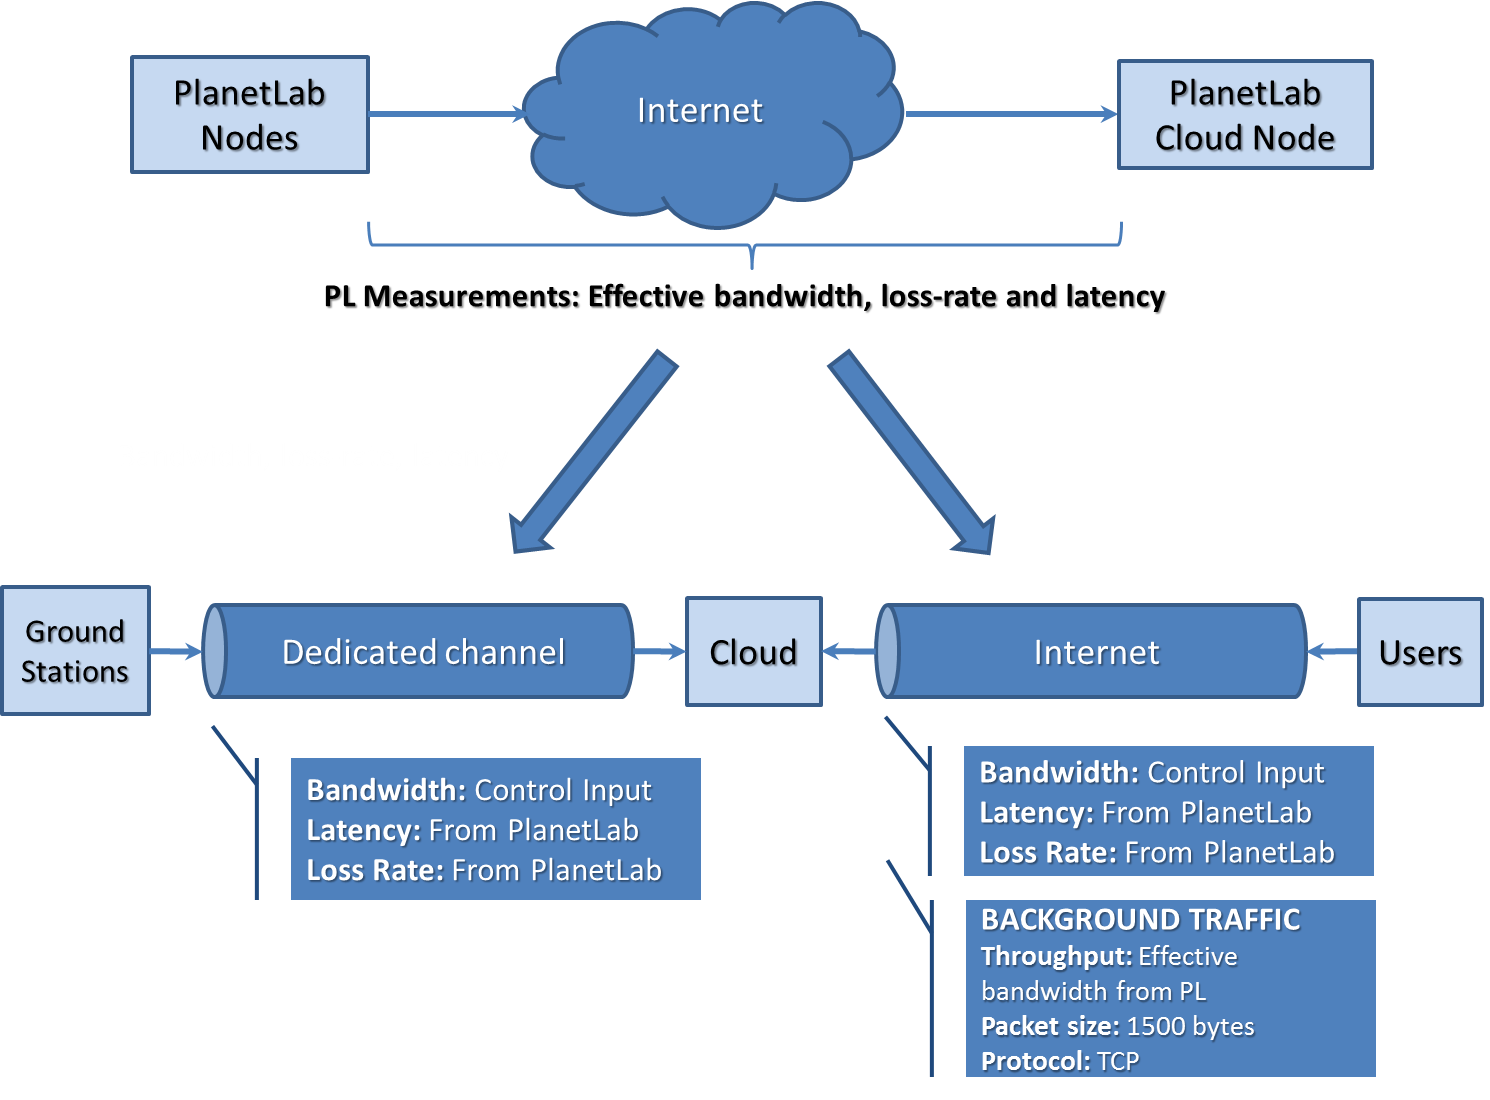
\includegraphics[width=5.22037in,height=3.85406in]{planetlab/modelled-links.png}
\caption{PlanetLab and modelled links equivalences}
\label{fig:ple-modelled-links}
\end{center}
\end{figure}


\subsubsection{System Modeling}

The real system was modeled into three main components: i) a network of ground stations acquiring imagery data from a constellation of optical satellites, ii) a cloud infrastructure that ingests the data from the ground stations, processes it, stores it and distributes it through web services and iii) end users around the world accessing to the web services offered. The system can be divided into two layers:

\begin{enumerate}

\item \emph{Layer 1} is constituted by 12 ground stations connecting with a cloud
  infrastructure. The ground stations and their location are depicted in Table~\ref{table:ple-groundstations-location}. Their locations and footprints are depicted in Figure~\ref{fig:intr-footprints}. The footprints represent the area in which the satellites can establish the communication with the ground stations.

\begin{table}[hp]
  \centering
  {\small
  


\begin{tabular}{p{.2\textwidth}p{.2\textwidth}}
  \tabheadformat
  \tabhead{Ground Station}   &
  \tabhead{Country of GS location}\\
\hline
\textit{Irkutsk}         & Russia \\
\hline
\textit{Puertollano}         & Spain \\
\hline
\textit{Svalbard}         & Norway \\
\hline
\textit{Troll}         & Antarctic \\
\hline
\textit{Chetumal}         & Mexico \\
\hline
\textit{Córdoba}         &  Argentina\\
\hline
\textit{Dubai}         &United Arab Emirates  \\
\hline
\textit{Kourou}         & French Guiana \\
\hline
\textit{Krugersdorp}         &South Africa  \\
\hline
\textit{Malaysia}         &  Malaysia\\
\hline
\textit{Prince Albert}         & Canada \\
\hline
\end{tabular}


% Local variables:
%   coding: utf-8
%   ispell-local-dictionary: "castellano8"
%   TeX-master: "main.tex"
% End:

  }
  \caption{Ground Station Location}
  \label{table:ple-groundstations-location}
\end{table}

% {\centering
% 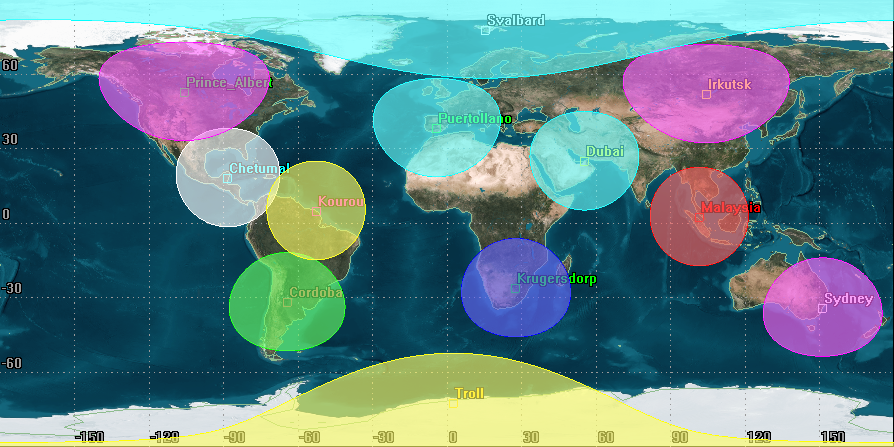
\includegraphics[width=5.37767in,height=2.68448in]{footprints.png} \par}

% {\centering\bfseries
% Figure\ 2\ Footprints of the ground stations.
% \par}

\item \emph{Layer 2} is constituted by the end users accessing the web services
  implemented in cloud. These users are distributed around the world and can be
  governments, emergency services, media and individuals among others.
\end{enumerate}

From the previous layers two networks can be identified: the network between the
ground stations and the cloud and the network between the end users and the
cloud. The system and the interconnections between components are depicted in
Figure~\ref{fig:ple-system-description}. The connections between the ground stations and end users with the
cloud are represented as arrows with different line types to represent that
every connection can have different characteristics and impairments. All the
connections are \ac{TCP}.

\begin{figure}[!h]
\begin{center}
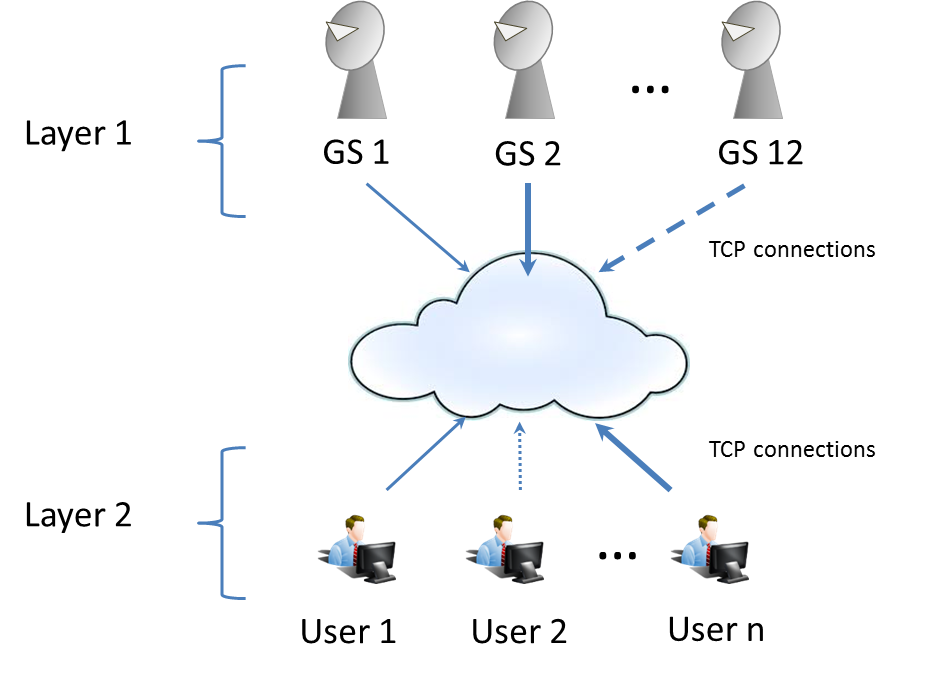
\includegraphics[width=3.35852in,height=2.41008in]{planetlab/system-description.png}

\caption{System description}
\label{fig:ple-system-description}
\end{center}
\end{figure}

The network was defined in function of the following representative impairments: \emph{effective bandwidth, latency and loss rate}. Thus, every link were represented in function of the previous impairments: effective bandwidth, latency, loss rate.
This system was implemented in \vw and \bonfire as depicted in
Figure~\ref{fig:ple-scheme-system}. The experiment in \pl was used to update the
network parameters connecting \vw and \bonfire.

\begin{figure}[!h]
\begin{center}
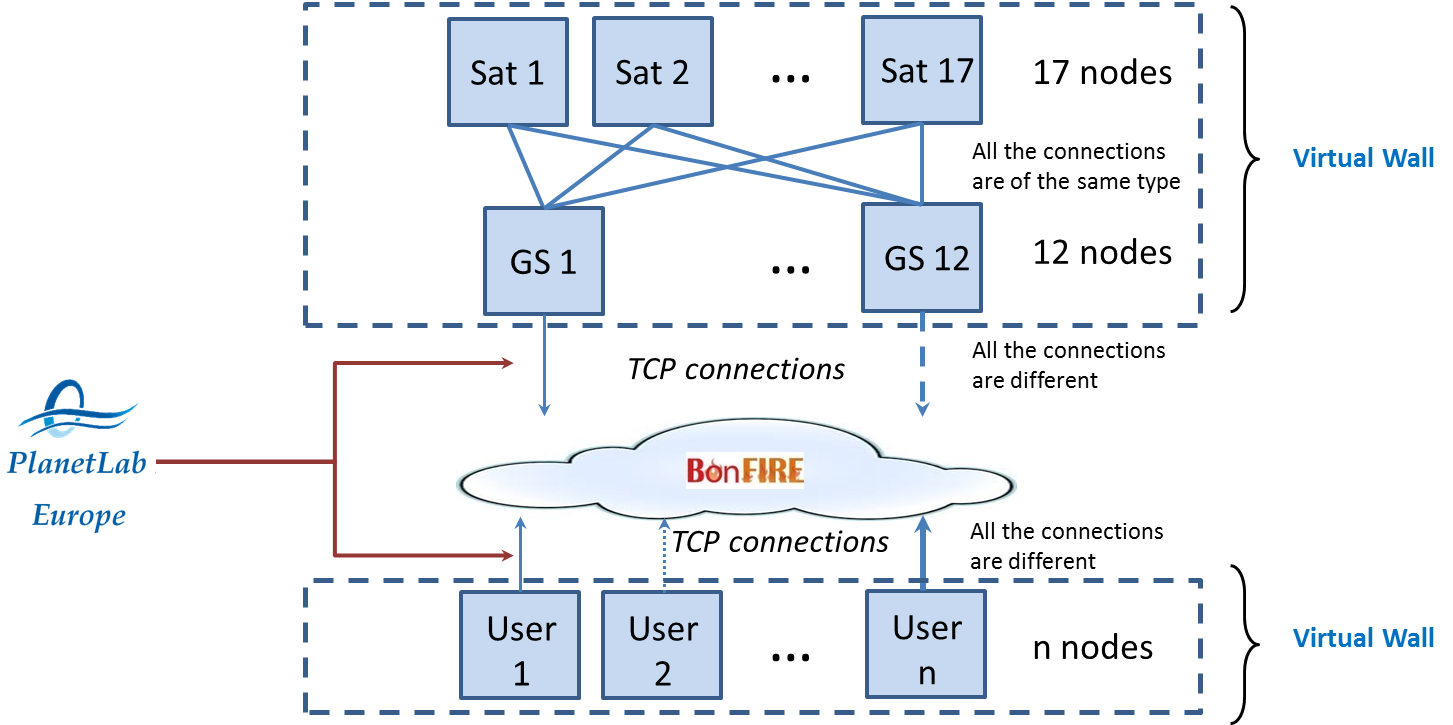
\includegraphics[width=5.48738in,height=2.73818in]{planetlab/schemeSystem.png}
\caption{Scheme of the system implemented in Geo-Cloud}
\label{fig:ple-scheme-system}
\end{center}
\end{figure}


\subsubsection{Network Design}

The model of the ground stations network, the cloud and the end users accessing
the web services provided was simplified to a set of interconnected nodes. The
network was divided into two layers connected by a central node representing the
cloud servers for similarity with the real system:
\begin{itemize}

\item \textbf{Layer 1:} it represents the connections between 12 nodes
  representing the ground stations and a central node representing the cloud
  servers. In \emph{PlanetLab Europe} and \emph{PlanetLab Central}, the nearest nodes to the
  real location of the ground stations were selected. For the central node, a
  node in \emph{INRIA} was chosen, since the \bonfire cloud has servers in the same
  location. This layer then represents the transfer of geodata acquired by the
  constellation of satellites from the ground stations in which the data is
  downloaded to the cloud. The network topology implemented is peer-to-peer,
  i.e. each node representing the ground stations is directly connected with the
  central node. In Table~\ref{tab:ple-tablelayer1-nodes} the \pl selected nodes for layer 1 and for the
  cloud central node are shown. The nodes are numbered in ascending order in
  function of the distance to the central node, i.e. the closest node is the
  number 0 and the furthest the 37.

% \begin{table}[hp]
%   \centering
%   {\small
%   
\begin{tabular}{c c c c c}
\tabheadformat
\tabhead{Ground Station} & \tabhead{Node Location} & \tabhead{Selected Node} & \tabhead{Site} & \tabhead{Node number}\\\hline
             Irkutsk\footnote{These ground stations are located in areas without nodes, the closest node has been selected.} & China & planetlab1.buaa.edu.cn & Beihang University & 24\\
             \hline
             Puertollano & Spain & Planetlab2.dit.upm.es & Universidad Polit\'{e}cnica Madrid  & 5\\
             \hline
             Svalbard & Norway & planetlab1.cs.uit.no & University of Tromso   & 14\\
             \hline
             Troll\footnote{These ground stations are located in areas without nodes, the closest node has been selected.} & New Zealand & planetlab1.cs.otago.ac.nz & University of Otago    & 37\\
             \hline
             Chetumal\footnote{These ground stations are located in areas without nodes, the closest node has been selected.} & USA & Planetlab1.eecs.ucf.edu & University of Central Florida & 22\\
             \hline
             C\'{o}rdoba & Argentina & planet-lab2.itba.edu.ar & Instituto Tecnol\'{o}gico Buenos Aires    & 34\\
             \hline
             Dubai\footnote{These ground stations are located in areas without nodes, the closest node has been selected.} & Israel & planet1.cs.huji.ac.il & The Hebrew University of Jerusalem   & 19\\
             \hline
             Kourou\footnote{These ground stations are located in areas without nodes, the closest node has been selected.} & Brazil & planetlab1.pop-pa.rnp.br & RNP  &26\\
             \hline
             Krugersdorp\footnote{These ground stations are located in areas without nodes, the closest node has been selected.} & Reunion Island (France) & lim-planetlab-1.univ-reunion.fr & Universite de La Reunion    & 28\\
             \hline
             Malaysia & Malaysia & planetlab1.comp.nus.edu.sg & National University of Singapore   & 32\\
             \hline
             Prince Albert & Canada & planetlab-2.usask.ca & University of Saskatchewan    & 21\\
             \hline
             Sidney & Australia & pl1.eng.monash.edu.au & National ICT Australia   & 36\\
             \hline
             Cloud\footnote{Node representing the cloud infrastructure.} & France & ple6.ipv6.lip6.fr & University Pierre et Marie Curie & N/A\\
             \hline
\end{tabular}
%   }
%   \caption{Ground Segment Nodes}
%   \label{tab:ple-tablelayer1-nodes}
% \end{table}


\item \textbf{Layer 2:} it represents the connection between the central node
  representing the cloud servers and the end users. 31 different nodes were
  selected in \emph{PlanetLab Europe} and \emph{PlanetLab} Central in 31 different countries
  around the world. This allows us to have a representative sample of global
  users accessing the web service
s. In this case, the network topology is also peer-to-peer. In Table~\ref{tab:ple-tablelayer2-nodes} the nodes selected for layer 2 are listed. We tried to increase the number of nodes in different countries, but during the execution of the experiment we did not find available PlanetLab nodes in the following countries: Austria, Cyprus, Denmark, Egypt, Ecuador, Iceland, India, Jordan, Mexico, Pakistan, Puerto Rico, Romania, Slovenia, Sri Lanka, Tunisia, Turkey, Venezuela, Uruguay and Taiwan.
\end{itemize}


% \begin{table}[hp]
%   \centering
%   {\small
%   
\begin{tabular}{c c c c c c }
\tabheadformat
\tabhead{Country} & \tabhead{Selected Node} & \tabhead{Number} &\tabhead{Country} & \tabhead{Selected Node} &\tabhead{Number}\\\hline
       Argentina  & planet-lab2.uba.ar                 & 35  &   Japan & planet1.pnl.nitech.ac.jp                &  31 \\\hline
       Australia & pl1.eng.monash.edu.au               & 36  &   Korea, Republic of & netapp7.cs.kookmin.ac.kr   &  27 \\\hline
       Belgium & rochefort.infonet.fundp.ac.be         & 2  &   The Netherlands & planetlab1.cs.vu.nl          & 4   \\\hline
       Brazil & planetlab1.pop-pa.rnp.br               & 26  &   New Zealand & planetlab1.cs.otago.ac.nz         &  37 \\\hline
       Canada & planetlab-2.usask.ca                   & 21  &   Norway & planetlab1.cs.uit.no                   &  14 \\\hline
       China & planetlab1.cqupt.edu.cn                 & 25  &   Poland & ple2.dmcs.p.lodz.pl                    &  13 \\\hline
       Czech Republic & planetlab1.cesnet.cz           & 8  &   Portugal & planet1.servers.ua.pt                & 11  \\\hline
       Finland & planetlab-1.research.netlab.hut.fi    & 17  &   Russian Federation & plab1.cs.msu.ru            & 20  \\\hline
       France & inriarennes2.irisa.fr                  & 0  &   Singapore & planetlab1.comp.nus.edu.sg          &   33\\\hline
       Germany & planetlab02.tkn.tu-berlin.de          & 6  &   Spain & dplanet2.uoc.edu                        &  3 \\\hline
       Greece & planetlab1.ionio.gr                    & 15  &   Sweden & planetlab2.s3.kth.se                   & 16  \\\hline
       Hong Kong & planetlab1.ie.cuhk.edu.hk           & 30  &   Switzerland & planetlab2.unineuchatel.ch        &  1 \\\hline
       Hungary & planet2.elte.hu                       & 12  &   Thailand & ple2.ait.ac.th                       & 29  \\\hline
       Ireland & planetlab-node-01.ucd.ie              & 10 &   United Kingdom & planetlab-2.imperial.ac.uk     &  9 \\\hline
       Israel & planetlab2.tau.ac.il                   & 18  &   United States & planetlab-04.cs.princeton.edu   & 23  \\\hline
       Italy & planet-lab-node1.netgroup.uniroma2.it   & 7  &           &    &\\\hline
\end{tabular}

%   }
%   \caption{User Nodes}
%   \label{tab:ple-tablelayer2-nodes}
% \end{table}


Figure~\ref{fig:ple-network-scheme} shows a scheme representing the network created in \pl. The
connections between the nodes are \emph{TCP}.

\begin{figure}[!h]
\begin{center}
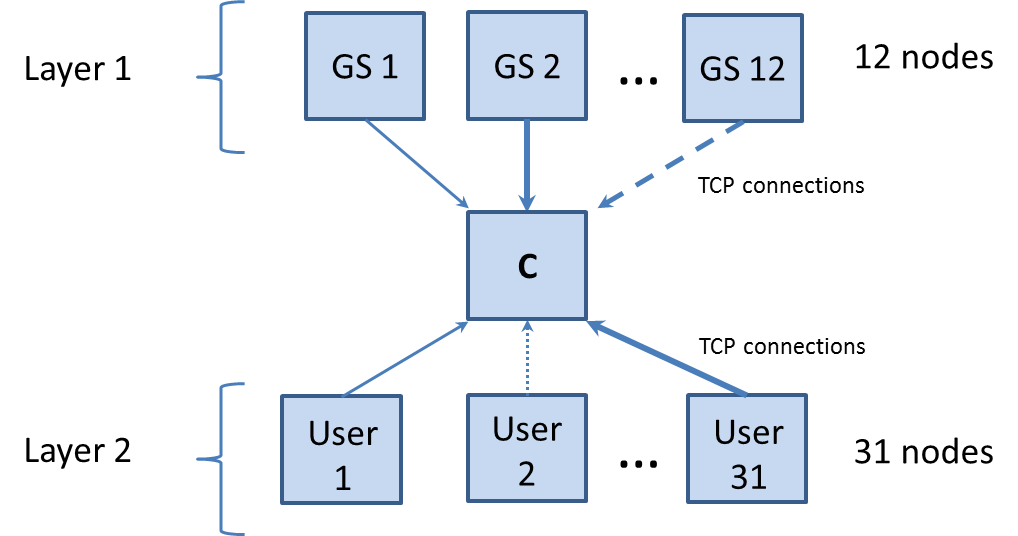
\includegraphics[width=4.01423in,height=2.11349in]{planetlab/network-scheme.png}

\caption{PlanetLab Network Scheme}
\label{fig:ple-network-scheme}
\end{center}
\end{figure}

\subsubsection{Experiment Design and Execution}

The experiment was designed to measure the impairments of the network. Those
impairments are required parameters in \vw to deploy a topology network in such
a testbed. Then, the latency, loss-rate and effective bandwidth were
measured. The deployment of the experiment was done with \nepi, in which
\emph{Iperf} and \emph{Ping} were implemented to measure the impairments. The
experiment consists of establishing communications between any node in layer 1
or layer 2 with the central node and measuring the previously described
impairments. 21600 trials were performed during 6 hours of the experiment execution in steps of one second for each pair of nodes, i.e. a node from layer 1 or 2 and the central node.

The software developed to measure the impairments is constituted of 6 scripts:
\begin{itemize}
\item Script to measure the effective bandwidth in the ground stations nodes: “bandwidthGS.py”.
\item Script to measure the effective bandwidth in the end users nodes: “bandwidthEndUser.py”
\item Script to measure the latency in the ground stations nodes: “latencyGS.py”.
\item Script to measure the latency  in the end users nodes: “latencyEndUser.py”
\item Script to measure the loss rate in the ground stations nodes: “lossRateGS.py”
\item Script to measure the loss rate in the end users nodes:
  “lossRateEndUser.py”

\end{itemize}

The pair of scripts that measure the same impairment are differentiated one from each other in the provisioning of the nodes. Those nodes representing the ground stations are manually selected, while the end users nodes are automatically provisioned by \nepi by indicating the country name as parameter. This parameter allows \nepi to select an available node in that country.

The previous six scripts were individually executed in a local host and they started their workflow.

\paragraph{The bandwidthGS.py script}~\\

The \emph{bandwidthGS.py}  script measures the effective bandwidth in the ground
stations nodes. When it is executed it carries out the next tasks:
\begin{enumerate}
\item Provisioning of the nodes that were manually selected.
\item Creation of the commands to be uploaded:
\begin{itemize}
\item In the cloud node:

\emph{timeout \%dm iperf -s -f m -i 1 -p \%d} \\
\emph{Timeout} is a command that executes a program during a specified time \%dm in
minutes. For this experiment $dm$ was chosen to be 6 hours.
\begin{itemize}
\item s indicates that \emph{Iperf} is executed in server mode
\item f m indicates the format to report the received data. In this case in $Mb$.
\item i 1 Periodic reports every 1 second
\item p \%d indicates the port to listen. In this case 20004.
\end{itemize}

\item In the ground station nodes:

\emph{iperf  -i 1 -f m -c \%s -t \%d -p \%d  -y c > node\%d.out}\\
\begin{itemize}
\item i 1 Periodic reports every 1 second.
\item f m indicates the format to report the received data. In this case in Mb.
\item c \%s indicates the server to establish the communication with.
\item t indicates the data transmission time. In this case 3600 seconds.
\item p \%d indicates the port to listen. In this case 20004.
\item y c> node\%d.out indicates that the report format is \ac{CSV}. The output file
  is node\%d.out, where \%d indicates the number of the node tested.
\end{itemize}
\end{itemize}

By default \emph{Iperf} is executed in \ac{TCP} mode.

\item Uploads the commands to the nodes
\item Executes the command in cloud
\item Executes the command in the rest of nodes
\item During the execution of the commands the data is collected
\item Finishes the execution of the commands
\item The data collected is retrieved
\item The resources are released.
\end{enumerate}

The flow diagram of the effective bandwidth measurements in the ground station nodes is depicted in Figure~\ref{fig:ple-workflow-ground-bandwidth}.

\paragraph{The bandwidthEndUser.py script}~\\

The \emph{bandwidthEndUser.py} script measures the effective bandwidth in the
end users nodes. When it is executed it carries out the next tasks:
\begin{enumerate}
\item Automatic provisioning of the nodes.
\item Tasks 2 to 9 of the \emph{bandwidthGS.py} script.
\end{enumerate}

The flow diagram of the effective bandwidth measurements in the end users nodes is depicted in Figure~\ref{fig:ple-workflow-enduser-bandwidth}.

\paragraph{The lossRateGS.py script}~\\

The \emph{lossRateGS.py}  script measures the loss rate in the ground stations
nodes. When it is executed it carries out the next tasks:

\begin{enumerate}
\item Provisioning of the nodes that were manually selected.
\item Creation of the commands to be uploaded:
\begin{itemize}
\item In the cloud node:

\emph{timeout \%dm iperf -s -f m -i 1 -p \%d -u} \\
\emph{Timeout} is a command that executes a program during a specified time \%dm in
minutes. For this experiment dm was chosen to be 6 hours.%65 minutos
\begin{itemize}
\item s indicates that \emph{Iperf} is executed in server mode
\item f m indicates the format to report the received data. In this case in $Mb$.
\item i 1 Periodic reports every 1 second
\item p \%d indicates the port to listen. In this case 20004.
\item u indicates that the \emph{Iperf} software is executed in \emph{UDP} mode.
\end{itemize}

\item In the ground station nodes:

\emph{iperf  -i 1 -f m -c \%s -t \%d -p \%d  -y c > node\%d.out}\\
\begin{itemize}
\item i 1 Periodic reports every 1 second.
\item f m indicates the format to report the received data. In this case in \emph{Mb}.
\item c \%s indicates the server to establish the communication with.
\item t indicates the data transmission time. In this case 3600 seconds.
\item p \%d indicates the port to listen. In this case 20004.
\item y c> node\%d.out indicates that the report format is \ac{CSV}. The output file
  is node\%d.out, where \%d indicates the number of the node tested.
\item u indicates that the \emph{Iperf} software is executed in \emph{UDP} mode.
\end{itemize}
\end{itemize}

By default \emph{Iperf} is executed in \ac{TCP} mode.

\item Uploads the commands to the nodes
\item Executes the command in cloud
\item Executes the command in the rest of nodes
\item During the execution of the commands the data is collected
\item Finishes the execution of the commands
\item The data collected is retrieved
\item The resources are released.
\end{enumerate}

The flow diagram of the loss rate measurements in the ground station nodes is
depicted in Figure~\ref{fig:ple-workflow-ground-bandwidth}.

\paragraph{The lossRateEndUser.py script}~\\

The \emph{lossRateEndUser.py} script measures the loss rate in the end users
nodes. When it is executed it carries out the next tasks:
\begin{enumerate}
\item Automatic provisioning of the nodes.
\item Tasks 2 to 9 of the \emph{lossRateGS.py} script.
\end{enumerate}
The flow diagram of the loss-rate measurements in the end users nodes is
depicted in Figure~\ref{fig:ple-workflow-enduser-bandwidth}.

\paragraph{The latencyGS.py script}~\\

The \emph{latencyGS.py}  script measures the latency  in the ground stations
nodes. When it is executed it carries out the next tasks:
\begin{enumerate}

\item Provisioning of the nodes that were manually selected.
\item Creation of the commands to be uploaded:

\emph{ping \%s -w \%d}
\begin{itemize}
\item \%s indicates the host to do ping
\item w \%d indicates the time of the ping execution.
\end{itemize}
\item Uploads the commands to the nodes
\item Executes the command in cloud
\item Executes the command in the rest of nodes
\item During the execution of the commands the data is collected
\item Finishes the execution of the commands
\item The data collected is retrieved
\item The resources are released.
\end{enumerate}

The flow diagram of the latency measurements in the ground station nodes is depicted in Figure~\ref{fig:ple-workflow-latency-ground}.

\paragraph{The latencyEndUser.py script}~\\

The \emph{latencyEndUser.py}  script measures the latency in the end users
nodes. When it is executed it carries out the next tasks:
\begin{enumerate}
\item Automatic provisioning of the nodes.
\item Tasks 2 to 9 of the \emph{latencyGS.py} script.
\end{enumerate}

The flow diagram of the latency measurements in the end users nodes is depicted
in Figure~\ref{fig:ple-workflow-latency-user}.

\begin{figure*}
\begin{center}
\subfloat[Flow diagram of the \emph{bandwidthEndUser.py} and \emph{lossRateEndUser.py} scripts]{ 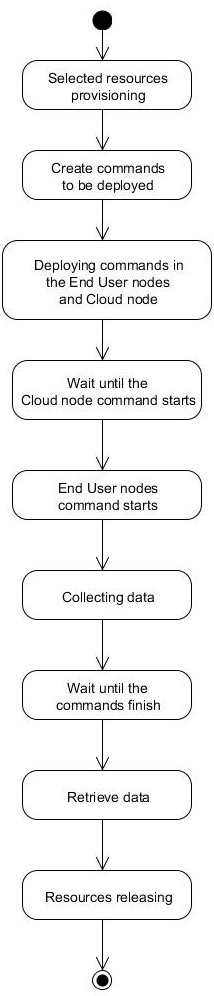
\includegraphics[width=0.2\textwidth]{planetlab/PLClient.jpg}
\label{fig:ple-workflow-enduser-bandwidth}}
\hspace{0.03\textwidth}
\subfloat[Flow diagram of the \emph{bandwidthGS.py} and \emph{lossRateGS.py} scripts]{ 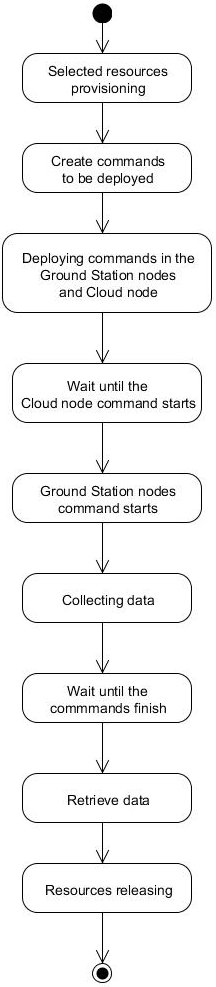
\includegraphics[width=0.2\textwidth]{planetlab/PLGS.jpg}
\label{fig:ple-workflow-ground-bandwidth}}
\hspace{0.03\textwidth}
\subfloat[Flow diagram of the \emph{latencyGS.py} script]{ 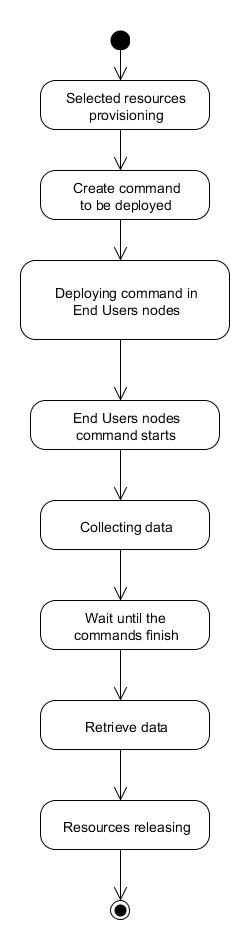
\includegraphics[width=0.2\textwidth]{planetlab/PLPINGClients.jpg}
\label{fig:ple-workflow-latency-user}}
\hspace{0.03\textwidth}
\subfloat[Flow diagram of the \emph{latencyEndUser.py} script]{ 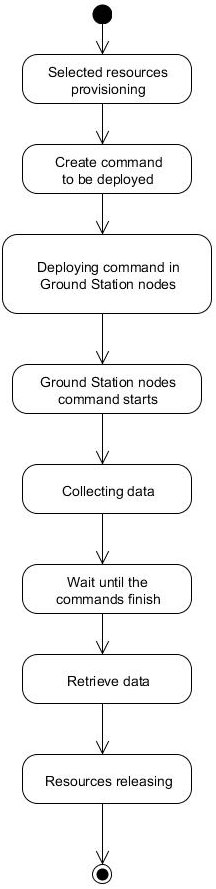
\includegraphics[width=0.2\textwidth]{planetlab/PLPINGGS.jpg}
\label{fig:ple-workflow-latency-ground}}
\end{center}
\end{figure*}



\section{PlanetLab Experiment Results}
\label{sec:pl-res}
During the execution of the \pl experiment (see Section~\ref{sec:planetlab}) 21600 communications were established between every node representing ground stations and users and the central node representing the cloud. The bandwidth, latency and loss rate were measured.
In Figure~\ref{fig:Bandwidth_gs_hist} the 21600 samples acquired in the communication between the node 22 and the central node during 6 hours of continuous execution are represented in a normalized histogram. The data accurately fits to a gaussian distribution with mean $3.28~Mbps$ and standard deviation $0.446~Mbps$. In Figure~\ref{fig:Latency_gs_hist} a normalized histogram of the measured latency is represented. It was fitted with a gaussian distribution with mean $154.210~ms$ and standard deviation $1.314~ms$. The loss rate between this node and the central node was obtained to be $0.0096$\%~\cite{Gonzalez2014}.
\begin{figure*}
\begin{center}
  \subfloat[Bandwidth of the node representing Chetumal ground station]{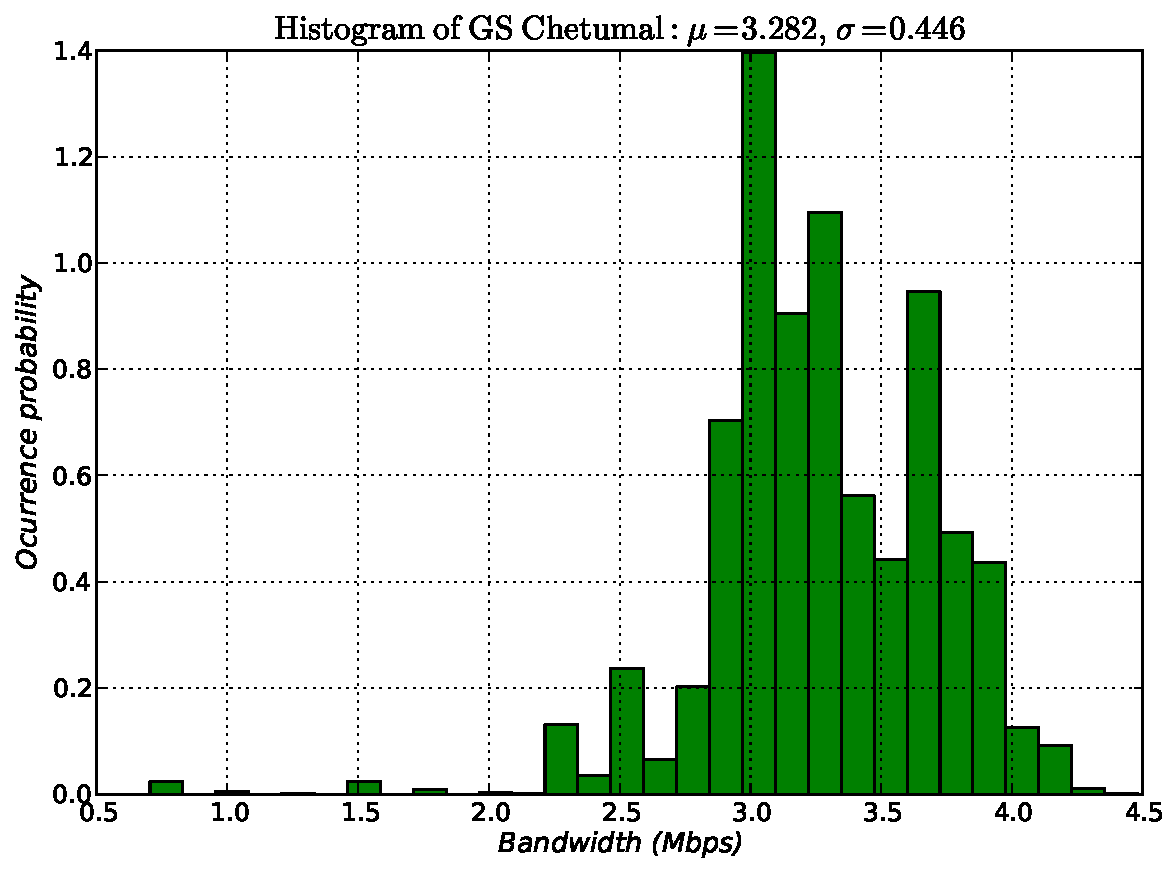
\includegraphics[scale=0.35]{resultsPL/IndividuallyGSHistChetumal.pdf}
 \label{fig:Bandwidth_gs_hist}}
\hspace{0.01\textwidth}
\subfloat[Latency of the node representing Chetumal ground
station]{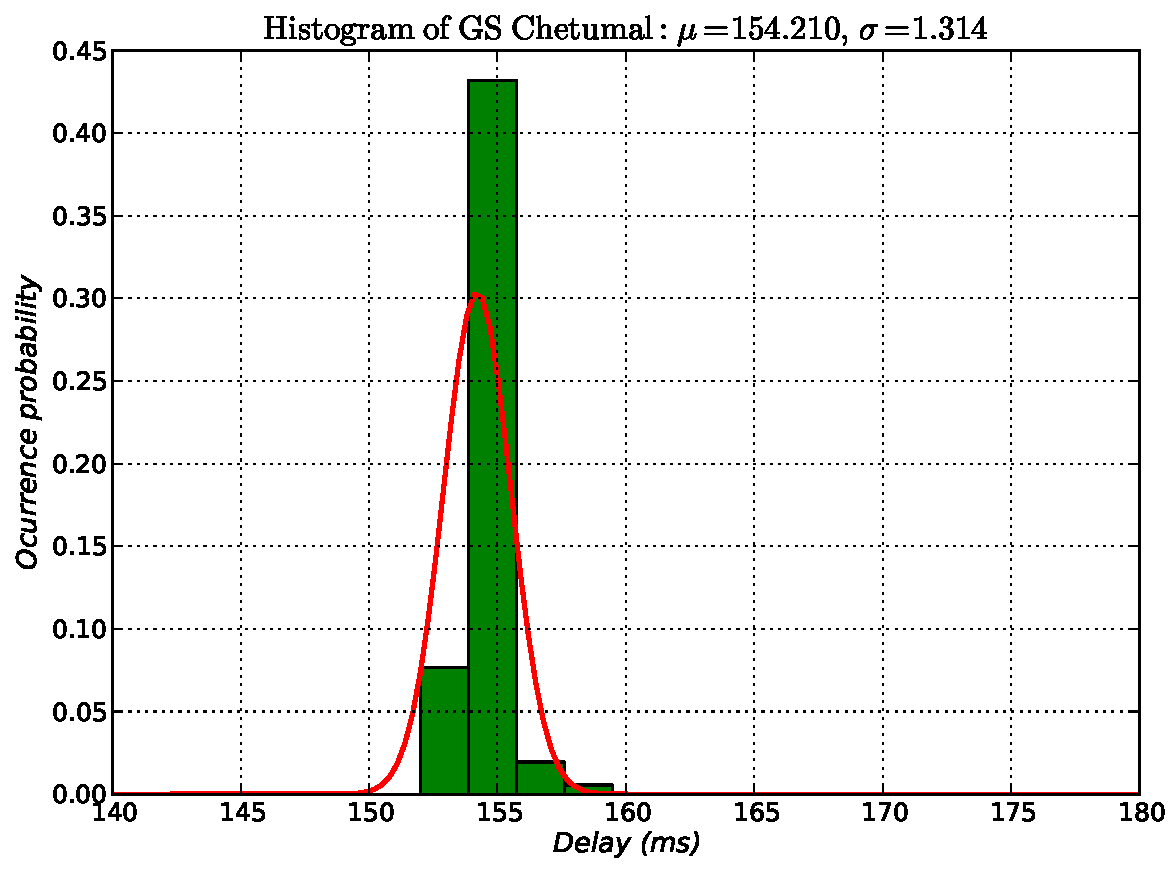
\includegraphics[scale=0.35]{resultsPL/DelayHistGSChetumal.pdf}
 \label{fig:Latency_gs_hist}}
\end{center}
\end{figure*}



The previous procedure was followed for the rest of the nodes. In
Figure~\ref{fig:bandwidth-plot} the mean and the standard deviation for each
node are depicted respectively. It can be observed that in general, the
bandwidth decreases when the distance between nodes increases. However the node
5 in Madrid presents a higher dispersion in the bandwidth value with respect to
the rest of nodes. It has a bandwidth of $15.2~Mbps$. The measurements were
fitted with different functions by using the least squares optimization
method. Exponential, polynomial, logarithm and hyperbolic functions were used to
fit the samples. For each fitted function the $R^2$ coefficient of
determination, which varies between 0 and 1, and indicates how well the
statistical distribution is fitted. The highest the value of the $R^2$, the
better the fitting. The following results were obtained: for exponential
function: $Bandwidth=4.655e^{-10^{-4}x}$,$R^2=0.5454$; for polynomial function
$Bandwidth=-3\cdot10^{-4}x+4.9444$, $R^2=0.3628$ and for logarithm function $Bandwidth=-1.519Ln(x)+15.325$, $R^2=0.4539$, where $x$ is the distance between any node and the central node in $km$. The bandwidth was obtained in $Mbps$. However, the hyperbolic function was the one that best fitted the distribution:
\begin{equation}\label{eq:bandwidth_fitting}
Bandwidth=184.91x^{-0.547};~R^2=0.582
\end{equation}

\begin{center}
\begin{figure}[h]
  \centering
  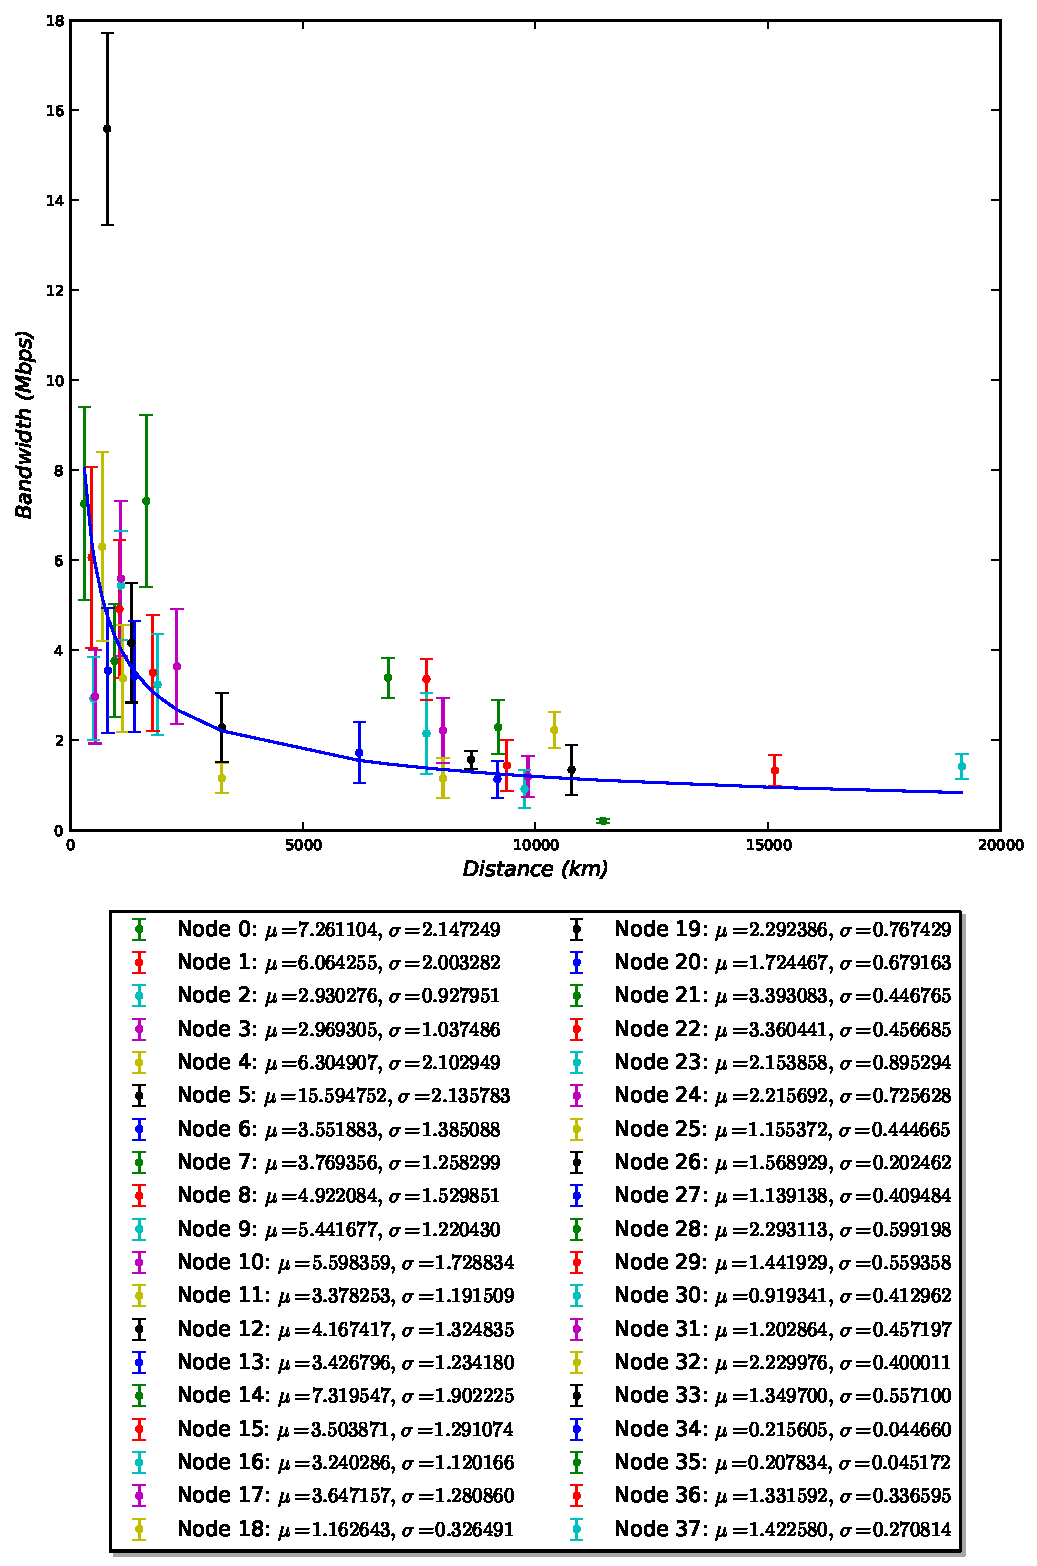
\includegraphics[scale=0.7]{resultsPL/bandwidthall.pdf}\\
  \caption{Bandwidth of all nodes} \label{fig:bandwidth-plot}
\end{figure}
\end{center}

Figure~\ref{fig:delay-plot} shows the mean and standard
deviation of the latency measured in all the nodes connecting the central node
in France. In this case the fitting used was a linear function. It accurately fitted the data distribution. The equation that approximated the data is the following:
\begin{equation}\label{eq:latency_fitting}
Latency=0.0228x+17.88;~R^2=0.8927
\end{equation}
The latency is obtained in $ms$ when the distance $x$ is introduced in $km$.


\begin{center}
\begin{figure}[h]
  \centering
  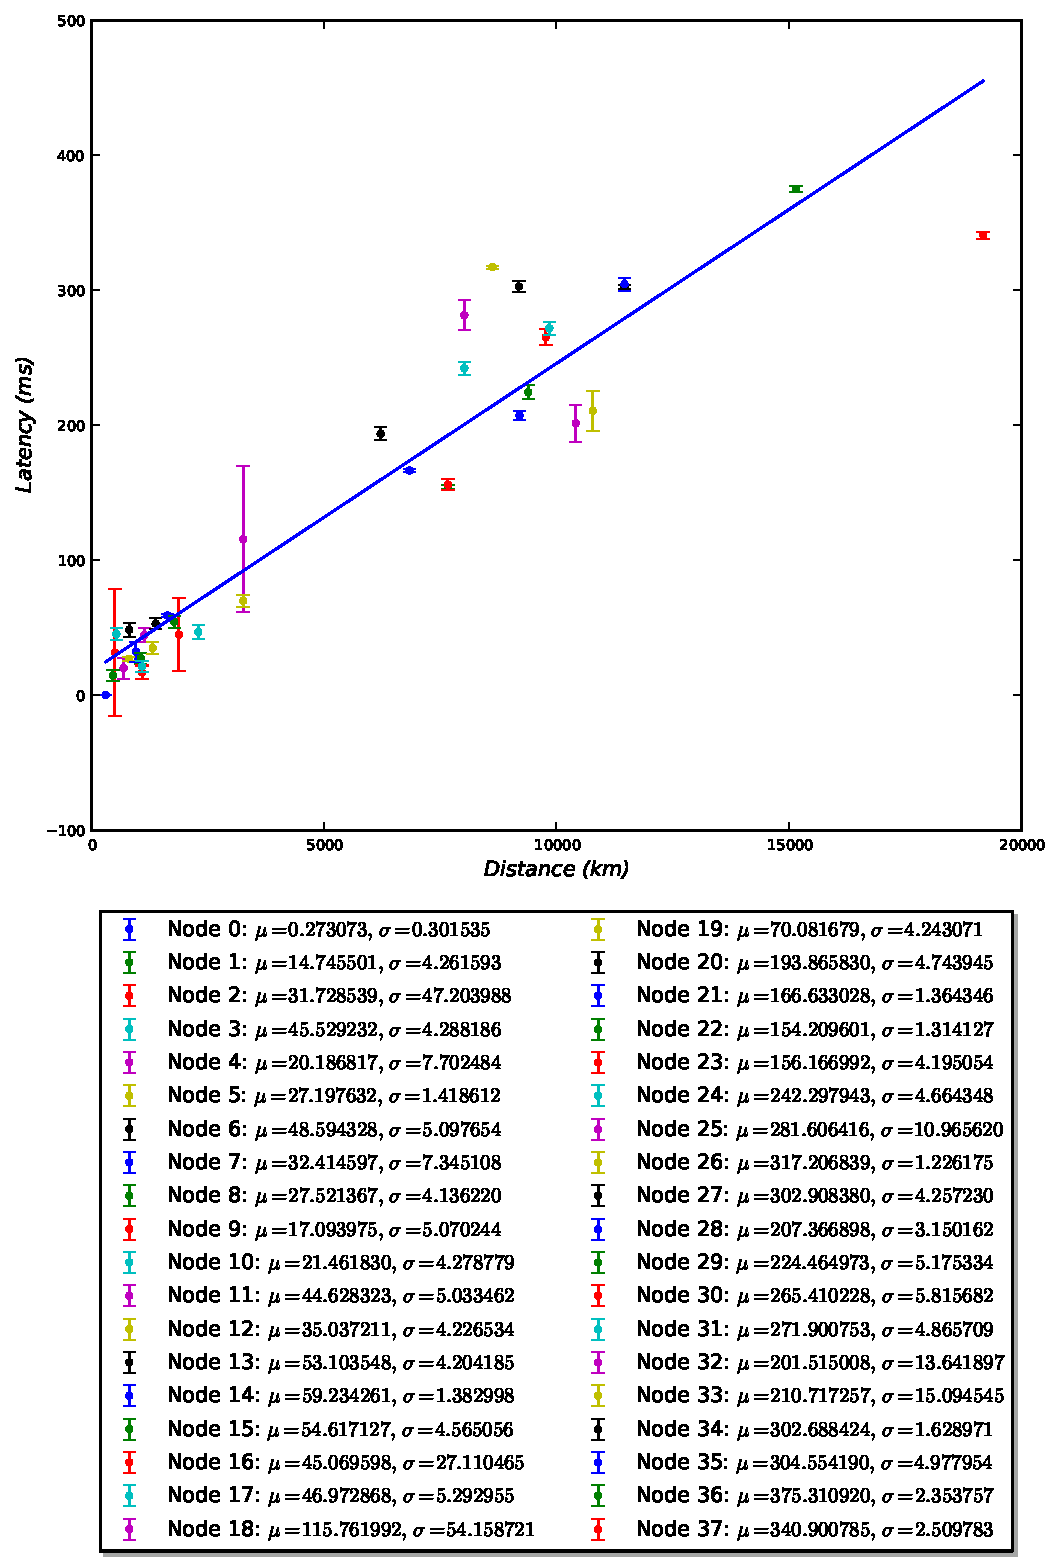
\includegraphics[scale=0.7]{resultsPL/DelayNodes.pdf}\\
  \caption{Latency of all nodes} \label{fig:delay-plot}
\end{figure}
\end{center}

Figure~\ref{fig:loss-rate-plot} shows the loss rate between any node and the central node during the whole execution of the experiment. In most of the communications the loss rate was under 0.2\%. Two cases are remarkable: on the one hand, between the node 20 in Russia and the central node 0\% of loss rate was measured, which means that no packets were lost; on the other hand, between Greece (node 16) and the central node, a loss rate of 15.68\% was measured, maybe because of interruptions in the network, overload of the server in Greece or routed network fails. The mean of the loss rates between all the communications was 0.053\% with a standard deviation of 0.097\% without considering the node in Greece in the calculations.

Table~\ref{anex:nodes-pl-results} summarizes the obtained measures. Column 5 and 6 show the mean and
the standard deviation of the bandwidth measured in all the nodes connecting the
central node in France. Column 7 and 8 also depict the mean and standard
deviation of the latency in the nodes. Finally, column 9 represents the measured
loss-rate between any node and the central node during the experiment.




\begin{center}
\begin{figure}[h]
  \centering
  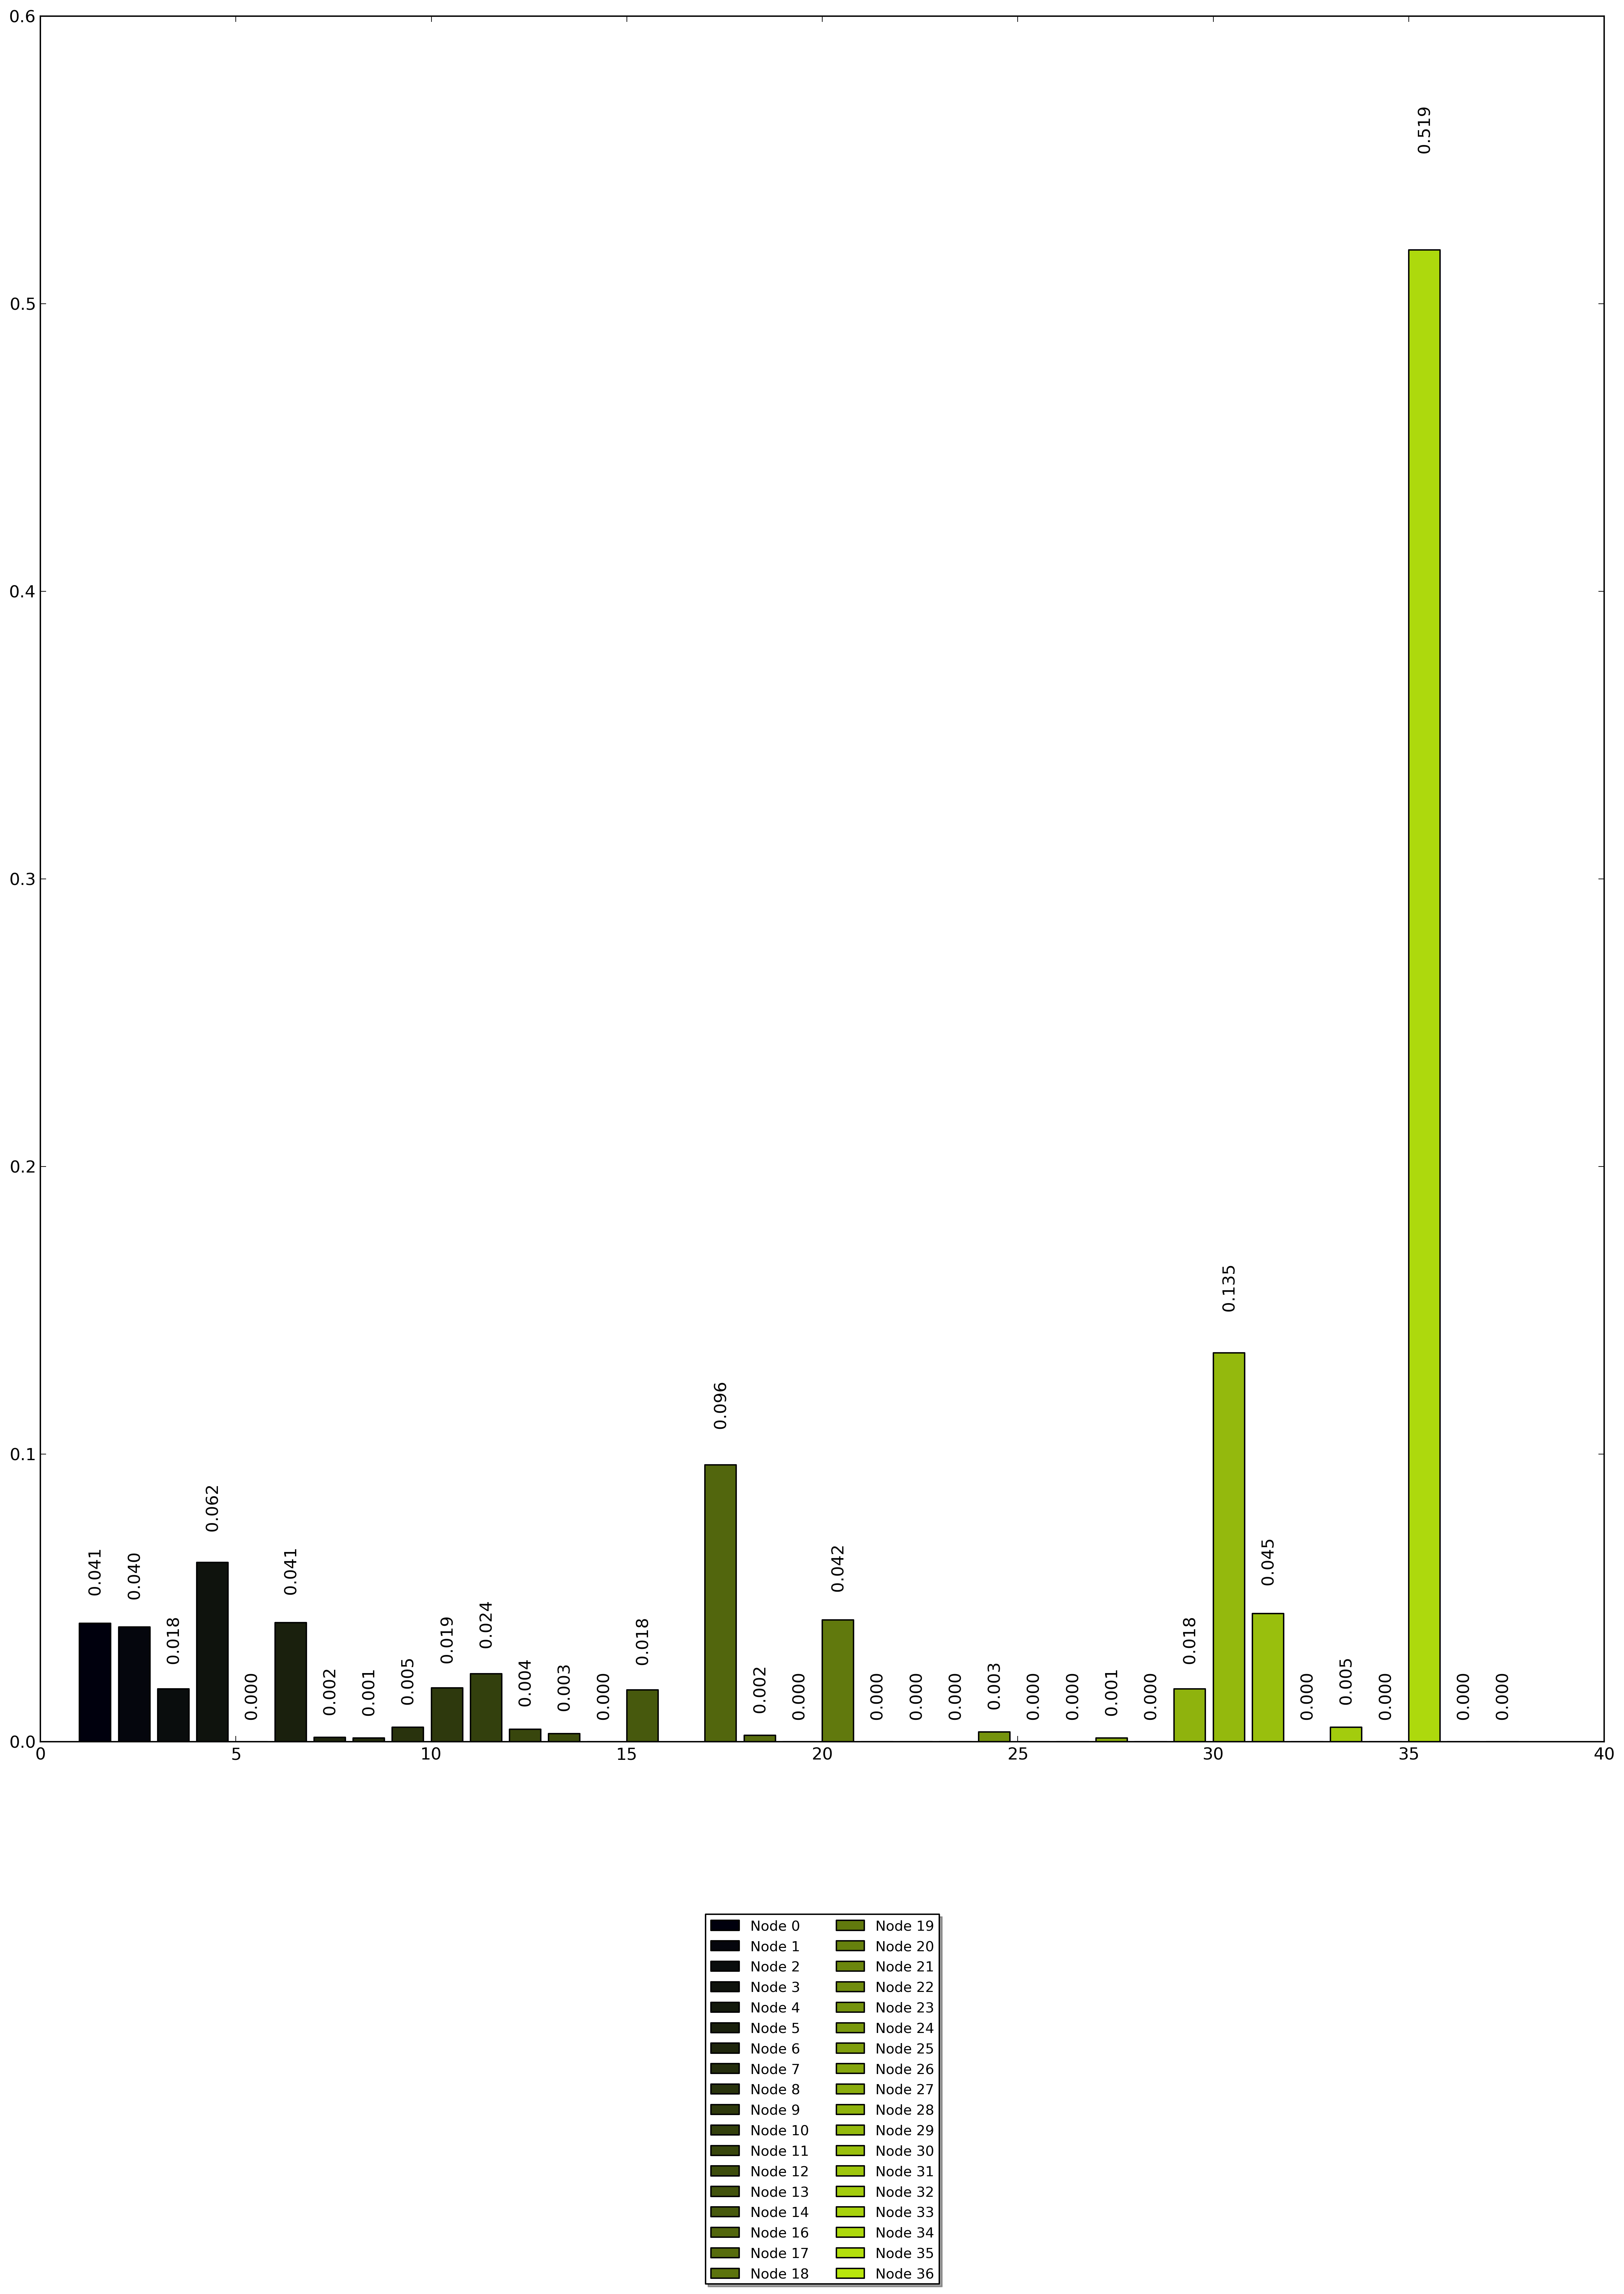
\includegraphics[scale=0.7]{resultsPL/Loss-rateALL.png}\\
  \caption{Bandwidth of all nodes.} \label{fig:loss-rate-plot}
\end{figure}
\end{center}

